% !TEX encoding = UTF-8 Unicode



\documentclass[10pt]{article}
\usepackage[utf8]{inputenc}
\usepackage[T1]{fontenc}
\usepackage[french]{babel}

\usepackage{amsmath}
\usepackage{amssymb}



% -------------------------------------
% Marges et dimensions papier
% -------------------------------------

\usepackage[ paperwidth=8.5in, paperheight=11in,
			 lmargin=1.25in, rmargin=1.25in, tmargin=1.25in, bmargin=1.25in]{geometry}


% -------------------------------------
%  Mise en page 
% -------------------------------------

\setlength{\parskip}{0.2cm}     % espace entre 2 paragraphes
\setlength{\parindent}{0.0cm}	  % retrait du premier mot de chaque paragraphe (alinéa)
%\usepackage[onehalfspacing]{setspace}   % espace entre les lignes d'un paragraphe


% ------------------------------
% Modules pour les mathématiques
% ------------------------------
\usepackage{amsmath}
\usepackage{amssymb}
%\usepackage{icomma}  % Les espaces en mode mathématique sont mieux gérés
\usepackage{graphicx}


% -------------------------------------
%  Modules divers
% -------------------------------------

\usepackage{float} % Pour avoir l'option H des tables et figures
\usepackage{enumerate}
\usepackage{graphicx}
\usepackage[colorlinks, linkcolor=blue, urlcolor=blue, citecolor=blue]{hyperref}


% -------------------------------------
% Paramètres pour la page titre
% -------------------------------------

\author{	
	Patrick Nzudom
     }
     
\title{Bloc 1}
\date{14 avril 2022}


% -------------------------------------
% Début du contenu
% -------------------------------------

\begin{document}

\maketitle

\rule{\linewidth}{.5pt}

\tableofcontents

\section{Bloc 1 - Et pourquoi pas prédire le futur?}


Grâce à la chaîne de Markov, ou modèle de Markov, je peux estimer le comportement futur des individus à l'aide de processus stochastiques, ou aléatoires. Selon un processus stochastique, seul le passé détermine l'évolution du processus ou la probabilité qu'un évènement ne se produise \cite{Markov}.


Dans ce bloc,  nous verrons comment simuler une chaîne de Markov avec \texttt{Python} et comment illustrer certaines de ses propriétés.  Dans les suite $(listeapprox)$,  il y aura une chaîne de Markov à espaces d'états $A$ et $B$ et de vecteurs d'état initial $S_0$ et $P_0$, pour deux situations différentes.


\subsection{Simulation d'une chaîne de Markov}

D'après mes connaissances, il n'y a pas de fonction toute faite, en \texttt{Python}, pour générer une chaîne de Markov à partir de sa matrice de transition. Toutefois, c'est possible de le faire et la méthode est située dans le livre de Vincent Vigon \cite{Pythonprobastat}.


Le premier exemple est le suivant: Un individu sans dettes a une possibilité sur trois de finir endetté, et lorsqu'un individu est endetté, il a une possibilité sur 6 de ne plus avoir de dettes.


Dans la première situation, l'ensemble d'état contient deux états possibles. Premièrement, celle où l'individu est endetté, puis finalement celle où l'individu est sans dettes. Je cherche la probabilité pour un individu endetté et un individu sans dettes de passer d'un état à un autre ou de rester dans le même état \cite{SituationDette}.

J'insère la figure représentant la situation que j'ai conçu au préalable à l'aide du site web overleaf.com

\begin{figure}[H]
	\centering
	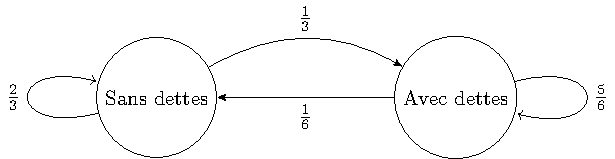
\includegraphics[scale=0.8]{dette.pdf}
	\caption{Probabilités qu'un individu soit endetté ou non}
\end{figure}

Pour représenter la chaîne de Markov, il faut définir l'ensemble d'état. Dans ce cas, il s'agit de :
$\Omega={\text{Sans dettes}, \text{Avec dettes}}$


Ensuite, je commence par créer la matrice de probabilités de transition $A$.


\[
        \begin{array}{c|cc}
	 & \text{Sans dettes} & \text{Avec dettes}\\
	\hline
	\text{Sans dettes} & 2/3 & 1/6\\
	\text{Avec dettes} & 1/3 & 5/6\\
	\end{array}
\]

Ensuite,  je crée le vecteur d'état initial du système $S_0$.


\begin{equation}
\label{eq:Vectinitial}
	\begin{bmatrix} 
	1\\
	0\\
	\end{bmatrix}
\end{equation}




Après une étape ou une journée, il faut multiplier le vecteur $S_0$ trouvé plus haut \eqref{eq:Vectinitial}  par $A$ pour trouver le vecteur d'état.
On obtient:


\begin{equation}
S_1 = (A)(S_0)= 	\begin{bmatrix} 
	2/3\\
	1/3\\
	\end{bmatrix}
	\quad
\end{equation}


Ainsi de suite, après deux étapes ou deux jours, on peut calculer le carré $A^2$ et puis multiplier le vecteur $S_0$ par $A^2$ pour trouver le vecteur d'état.

En effet, il y a deux méthodes d'effectuer ce calcul. On peut calculer 
\[
A_2 = (A_0)(A_1)
\]
\[
A_2 = (A^2)(S_0)
\]

Ce qui donne des probabilités égales:

\[
A_2 = (A^2)(S_0) = 	\begin{bmatrix} 
	1/2\\ 
	1/2\\
	\end{bmatrix}
	\quad
\]



Après un an, j'obtiens de la même manière:

\[
A_{365} = (A^{365})(S_0) = 	\begin{bmatrix} 
	1/3\\ 
	2/3\\
	\end{bmatrix}
	\quad
\]
Pour savoir si les puissances de la matrice de transition converge, on continue les calculs de celles-ci en les multipliant par le vecteur d'état initial du système $S_0$.
Après un an et plus, on remarque, grâce à python et la suite $(listeapprox)$, qu'une personne commençant endettée ou pas, elle aura 2 chances sur 3 de finir endettée.

\subsection{Simulation d'une autre chaîne de Markov}


Dans la seconde situation, le sujet à l'étude est les passes que se font trois joueurs de hockey entre eux. Il y a le joueur A, le joueur B, et le joueur C \cite{hockey}. La chaîne de Markov est celle de la probabilité pour qu'un joueur passe la rondelle à un autre.

\begin{figure}[H]
	\centering
	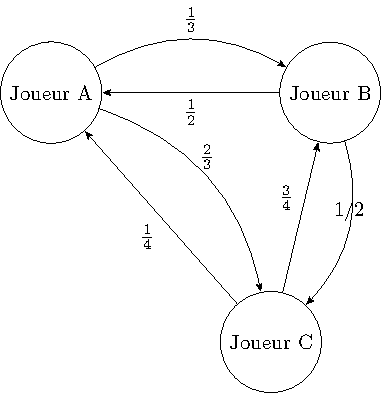
\includegraphics[scale=0.8]{pichockey.pdf}
	\caption{Probabilités qu'un joueur fasse la passe à un autre}
\end{figure}

$\Omega={A, B, C}$


Ensuite, je commence par créer la matrice de probabilités de transition $B$.
J'obtiens:


\[
        \begin{array}{c|ccc}
	& A & B & C\\
	\hline
	A & 0 & 1/3 & 2/3\\
	B & 1/2 & 0 & 1/2\\
	C & 1/4 & 3/4 & 0\\
	\end{array}
\]



On peut interpréter cette matrice de la façon suivante : Lorsque le joueur A a la rondelle, il y a une chance sur trois qu'il la passe au joueur B et 2/3 sont les probabilités qu'il la passe au joueur C.
Lorsque le joueur B a la rondelle, il y a une chance sur deux qu'il la passe au joueur a et 1/2 sont les probabilités qu'il la passe au joueur C, et ainsi de suite.


Ensuite,  je crée le vecteur d'état initial du système $P_0$.

\[
P_0 =	\begin{bmatrix} 
	0\\ 
	1\\ 
	0\\
	\end{bmatrix}
	\quad
\]

Après une étape ou une passe, on peut multiplier le vecteur $P_0$ par $B$ pour trouver le vecteur d'état.
On obtient:

\[
P_1 = (B)(P_0) =	\begin{bmatrix} 
	1/3\\
	0\\ 
	3/4\\
	\end{bmatrix}
	\quad
\]

Ainsi de suite, après trois étapes ou trois passes, on peut calculer le cube $B^3$ et puis multiplier le vecteur $P_0$ par $B^3$ pour trouver le vecteur d'état.
Cela donne les probabilités suivantes, pour chaque joueur d'avoir la rondelle:


\[
	\begin{bmatrix} 
	0.236111111111111 & 0.291666666666667 & 0.53125\\
	\end{bmatrix}
	\quad
\]


De la même manière, dans une situation hypothétique où les trois joueurs A, B et C se seraient fait 100 passes les probabilités pour chacun des joueurs d'avoir la rondelle sont égales:


\[
	\begin{bmatrix} 
	0.3636363636364 & 0.3636363636364 & 0.3636363636364\\
	\end{bmatrix}
	\quad
\]


Bien qu'ils n'aient pas été utilisés dans ce bloc, les vecteur propres et les valeurs propres sont des notions intéressantes en relation avec les chaînes de Markov.

\nocite{*}
\bibliographystyle{plain}
\bibliography{biblioMath}

\end{document}
